%\documentclass[dvips, intlimits, 8pt, unicode]{beamer} %для tex -> dvi -> ps -> pdf
\documentclass[pdf, 12pt]{beamer} %Для Latex2Pdf  tex -> pdf
%В качестве размера лучше использовать 9pt
%dvips нужно использовать только если использовать построение слайдов через PostScript
%intlimits - стиль для пределов интегралов (по желанию)
%unicode - обязательно

%Пакеты для русского языка
\usepackage[T2A]{fontenc}
\usepackage[utf8]{inputenc}
\usepackage[english,russian]{babel}
%Пакет для вставки рисунков
\usepackage{graphicx}

\def\Blue#1{\textcolor{blue}{#1}}

\usepackage{textcomp}
\usepackage{tikz}
\usepackage{times}
\usepackage{mathptmx}

\def\rmdefault{ftm}
\def\sfdefault{ftx}
\def\ttdefault{fer}
\DeclareMathAlphabet{\mathbf}{OT1}{ftm}{bx}{it} % bx/it or bx/m

%AMS TEX значки и пр.
\usepackage{amsfonts}
\usepackage{amsbsy}
\usepackage{amssymb}
\usepackage{amsthm}
\usepackage{wrapfig}

\usetheme{default}

% Удаляем навигационную панель
\setbeamertemplate{navigation symbols}{}

% Устанавливаем поля (по умолчнанию - 1 см)
\setbeamersize{text margin left=0.5cm, text margin right=0.25cm}

%Более крупный шрифт для подзаголовков титульного листа
\setbeamerfont{institute}{size=\normalsize}

%Задание команды (\bluetext) для выделения конкретным (синим) цветом
%\alert - выделение цветом выбранной "темы"
\setbeamercolor{bluetext_color}{fg=blue}
\newcommand{\bluetext}[1]{{\usebeamercolor[fg]{bluetext_color}#1}}

%Если используется последовательное появление пунктов списков на слайде
%(не злоупотребляйте в слайдах), чтобы
%еще непоявившиеся пункты были все-таки немножко видны.
\setbeamercovered{transparent}

% Путь к файлам с иллюстрациями
\graphicspath{{pics/}}

\newcommand{\insertpicc}[2]{
	\begin{figure}[H]
		\includegraphics[width=1\textwidth]{{pics/#1}}
		\caption{#2}
	\end{figure}
}

\newcommand{\insertpdf}[1]{
	\setlength{\voffset}{0cm}
	\setlength{\hoffset}{0cm}
	\includepdf[pages=-]{pics/#1}
	\setlength{\voffset}{\originalVOffset}
	\setlength{\hoffset}{\originalHOffset}
}

\newcommand{\myref}[2]{\href{#1}{\textcolor{blue}{#2}}}

\begin{document}

\begin{frame}
\frametitle{История развития региона}
\begin{columns}
\column{0.5\textwidth}
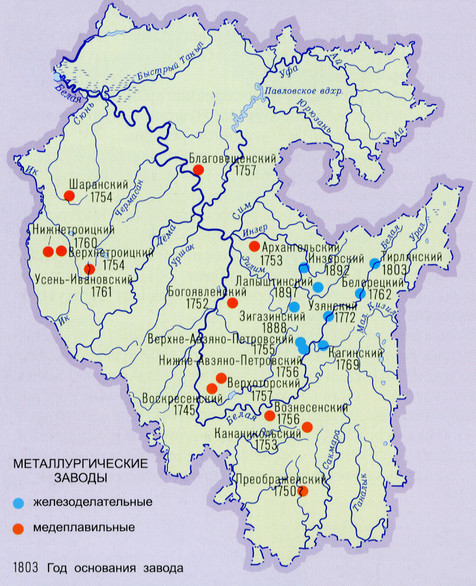
\includegraphics[width=1\linewidth]{pics/sasha/factories_18-19}

\column{0.5\textwidth}
Присоединение территорий республики завершилось к середине XVII века. \\[10pt]

Вторая половина XVII -- массовые восстания. 1773-1775 гг -- Крестьянская война. \\[10pt]

Со второй половины XVIII века начинают сооружаться заводы. \\[10pt]

20 марта 1919 г. -- создана Башкирская Автономная Советская Республика. 
\end{columns}
\end{frame}
%%%%%%%%%%%%%%%%%%%%%%%%%%%%%%%%%%%%%%%%%%%%%%%%%%%%%%%%%%%%%%%%%%%%

%%%%%%%%%%%%%%%%%%%%%%%%%%%%%%%%%%%%%%%%%%%%%%%%%%%%%%%%%%%%%%%%%%%%
\begin{frame}
\frametitle{История развития региона}

В 1920-30-е годы -- рост промышленного производства. 
\begin{center}
\begin{tabular}{|c|c|c|c|c|c|c|c|}
\hline 
Год & 1913 & 1940 & 1950 & 1960 & 1970 & 1980 & 1990 \\ 
\hline 
Темпы роста,\% & 1,0 & 10 & 41 & 186 & 478 & 983 & 1221 \\ 
\hline 
\end{tabular} 
\end{center}

1941 1945 гг. – Великая Отечественная война. Башкортостан стал одним из важнейших регионов перебазирования промышленности страны.

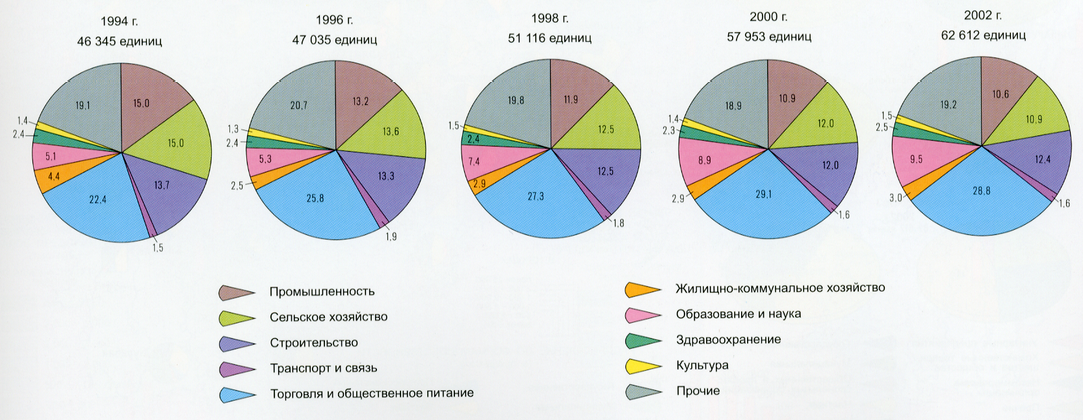
\includegraphics[width=1\linewidth]{pics/sasha/industries}

\end{frame}
%%%%%%%%%%%%%%%%%%%%%%%%%%%%%%%%%%%%%%%%%%%%%%%%%%%%%%%%%%%%%%%%%%%%

%%%%%%%%%%%%%%%%%%%%%%%%%%%%%%%%%%%%%%%%%%%%%%%%%%%%%%%%%%%%%%%%%%%%
\begin{frame}
\frametitle{Отраслевая и территориальная структура экономики}
\begin{columns}
\column{0.5\textwidth}
Центры промышленного производства: 
\begin{itemize}
\item Уфа 
\item Стерлитамак 
\item Салават 
\item Ишимбай 
\item Нефтекамск 
\end{itemize}

\column{0.4\textwidth}
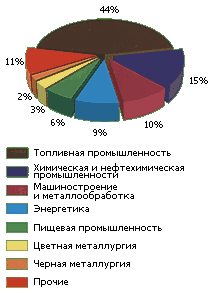
\includegraphics[width=1\linewidth]{pics/sasha/promstruct}
\end{columns}
\end{frame}
%%%%%%%%%%%%%%%%%%%%%%%%%%%%%%%%%%%%%%%%%%%%%%%%%%%%%%%%%%%%%%%%%%%%

%%%%%%%%%%%%%%%%%%%%%%%%%%%%%%%%%%%%%%%%%%%%%%%%%%%%%%%%%%%%%%%%%%%%
\begin{frame}
\frametitle{Отраслевая и территориальная структура экономики}

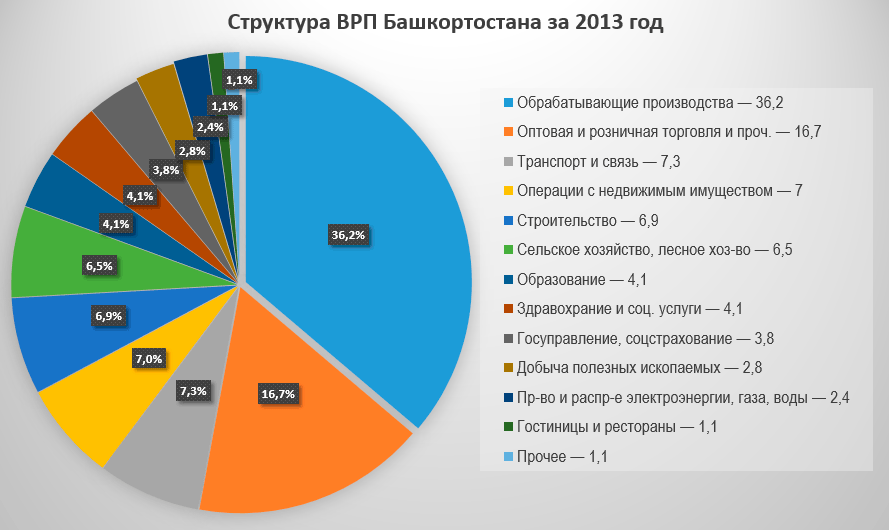
\includegraphics[width=1\linewidth]{pics/sasha/vrp} 

\end{frame}
%%%%%%%%%%%%%%%%%%%%%%%%%%%%%%%%%%%%%%%%%%%%%%%%%%%%%%%%%%%%%%%%%%%%

%%%%%%%%%%%%%%%%%%%%%%%%%%%%%%%%%%%%%%%%%%%%%%%%%%%%%%%%%%%%%%%%%%%%
\begin{frame}
\frametitle{Отраслевая и территориальная структура экономики}

$\blacktriangleright$ Нефтедобыча и нефтехимическая промышленность\\[2pt]

В республике разведано 191 месторождение нефти и газа, из них в разработке находится 161 месторождение. \\[2pt]
Ведущее нефтегазодобывающее предприятие Башкирии — ПАО «Акционерная нефтяная компания „Башнефть“». \\[5pt]

$\blacktriangleright$ Машиностроение и металлообработка
\begin{itemize}
\item производство оборудования для предприятий нефтедобычи, нефте- и газопереработки, химии и нефтехимии: г. Ишимбай, г. Салават
\item вертолестроение: г. Кумертау
\item производство автобусов: г. Нефтекамск 
\item производство троллейбусов: г. Уфа 
\item производство вездеходов: г. Ишимбай
\end{itemize}

\end{frame}
%%%%%%%%%%%%%%%%%%%%%%%%%%%%%%%%%%%%%%%%%%%%%%%%%%%%%%%%%%%%%%%%%%%%

%%%%%%%%%%%%%%%%%%%%%%%%%%%%%%%%%%%%%%%%%%%%%%%%%%%%%%%%%%%%%%%%%%%%
\begin{frame}
\frametitle{Отраслевая и территориальная структура экономики}
\begin{columns}
\column{0.5\textwidth}
$\blacktriangleright$ Пищевая промышленность\\[20pt]
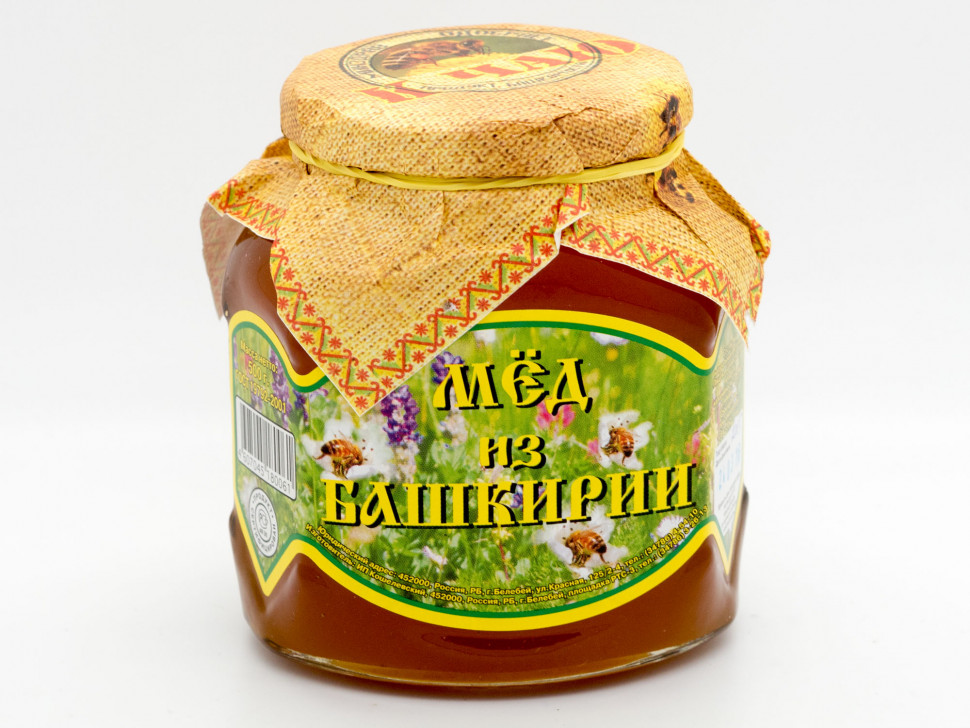
\includegraphics[width=1\linewidth]{pics/sasha/honey}

\column{0.5\textwidth}
$\blacktriangleright$ Энергетика\\[2pt]
\begin{itemize}
\item ТЭК: 50\% общерегионального объёма отгруженной продукции, 70\% полученной прибыли, 40\% поступлений в бюджет республики, более 30\% инвестиций в основной капитал и 80\% валютных поступлений
\item 31 электростанция
\item 3 солнечные электростанции
\end{itemize}
\end{columns}
\end{frame}
%%%%%%%%%%%%%%%%%%%%%%%%%%%%%%%%%%%%%%%%%%%%%%%%%%%%%%%%%%%%%%%%%%%%

%%%%%%%%%%%%%%%%%%%%%%%%%%%%%%%%%%%%%%%%%%%%%%%%%%%%%%%%%%%%%%%%%%%%
\begin{frame}
\frametitle{Отраслевая и территориальная структура экономики}

$\blacktriangleright$ Сельское хозяйство
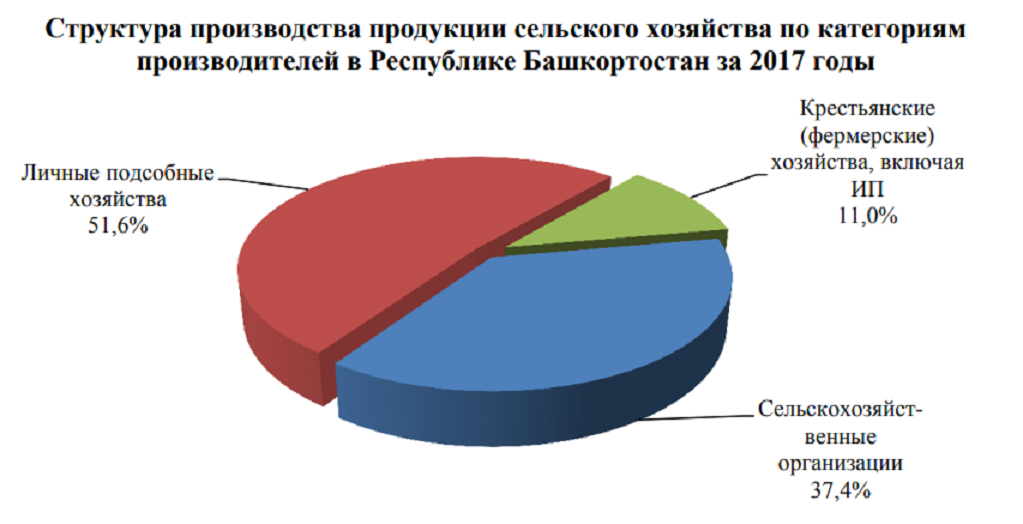
\includegraphics[width=1\linewidth]{pics/sasha/agriculture_struct}

\end{frame}
%%%%%%%%%%%%%%%%%%%%%%%%%%%%%%%%%%%%%%%%%%%%%%%%%%%%%%%%%%%%%%%%%%%%

%%%%%%%%%%%%%%%%%%%%%%%%%%%%%%%%%%%%%%%%%%%%%%%%%%%%%%%%%%%%%%%%%%%%
\begin{frame}
\frametitle{Отраслевая и территориальная структура экономики}

$\blacktriangleright$ Торговля\\[20pt]
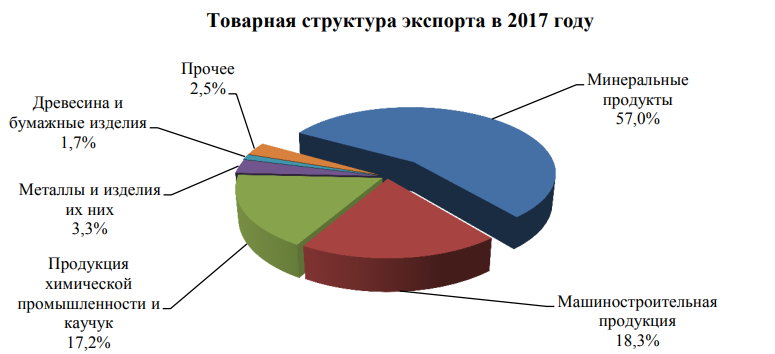
\includegraphics[width=1\linewidth]{pics/sasha/export}

\end{frame}
%%%%%%%%%%%%%%%%%%%%%%%%%%%%%%%%%%%%%%%%%%%%%%%%%%%%%%%%%%%%%%%%%%%%

%%%%%%%%%%%%%%%%%%%%%%%%%%%%%%%%%%%%%%%%%%%%%%%%%%%%%%%%%%%%%%%%%%%%
\begin{frame}
\frametitle{Отраслевая и территориальная структура экономики}

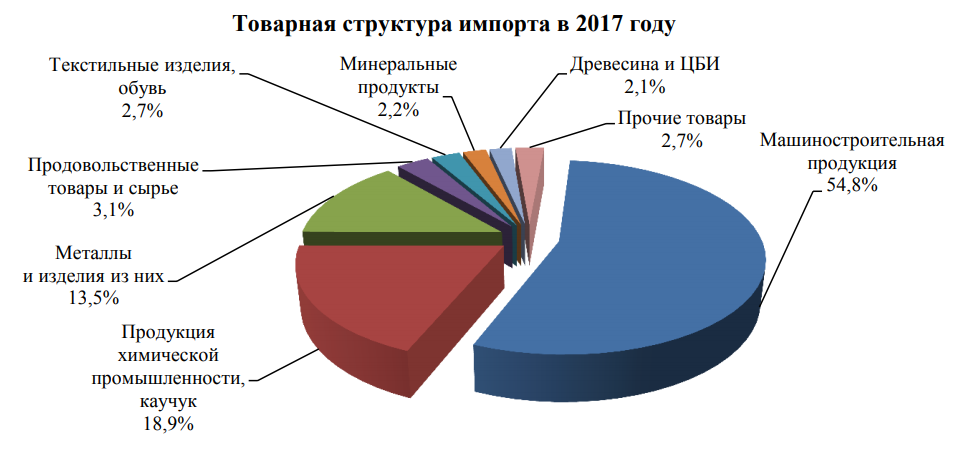
\includegraphics[width=1\linewidth]{pics/sasha/import}

\end{frame}
%%%%%%%%%%%%%%%%%%%%%%%%%%%%%%%%%%%%%%%%%%%%%%%%%%%%%%%%%%%%%%%%%%%%


\begin{frame} 
\frametitle{Макроэкономический анализ. Цели работы}

\begin{enumerate}
	\item Определить динамику ВРП.
	\item Оценить уровень безработицы в регионе, а так же конкретные отрасли с недостатком или переизбытком кадров.
	\item Собрать статистику по размерам оплаты труда в различных отраслях экономики.
	\item Сравнить уровни цен на различные категории товаров с другими регионами.
	\item Оценить демографическую ситуацию в регионе.
\end{enumerate}

\end{frame}

\begin{frame} 
\frametitle{Основной источник}

\begin{center}
\Large{БашкортостанСтан: \myref{http://bashstat.gks.ru/}{http://bashstat.gks.ru/}}
\end{center}

\end{frame}

\begin{frame} 
\frametitle{Распределение ВРП по отраслям}

\insertpicc{slava/vrp-2017.png}{Динамика ВРП на душу населения в рублях}

\end{frame}

\begin{frame} 
\frametitle{Распределение ВРП по отраслям}

Отрасли, доля ВРП которых составляет меньше 1 процента:
\begin{itemize}
	\item Водоснабжение, водоотведение, сбор отходов, ликвидация загрязнений
	\item Деятельность финансовая и страховая
	\item Деятельность в области культуры, спорта и развлечений
\end{itemize}

Доля остальных отраслей, включая образование, научную и техническую деятельность и здравоохранение составляет от 1 до 5 процентов.

\end{frame}

\begin{frame}
\frametitle{Динамика ВРП}
\insertpicc{slava/vrp-dynamics.png}{Динамика ВРП на душу населения в рублях}
\end{frame}

\begin{frame}
\frametitle{Факты}
\begin{itemize}
	\item Уровень безработицы на 2017 г. составил 5.6\%.
	\item Средняя заработная плата в январе 2019 года составила 30357,7.
	\item Средняя заработная плата по России в 2018 составила 43400
\end{itemize}
\end{frame}

\begin{frame}
\frametitle{Востребованность профессий. Нехватка кадров.}
Рабочие профессии, требующие квалификации и специальных навыков. Например:\\ автоэлектрик, машинист экскаватора, монтажник, оператор станков с программным управлением, сварщик, слесарь, токарь, электрик и т. д.
\end{frame}

\begin{frame}
\frametitle{Востребованность профессий. Переизбыток кадров.}
Должности служащих. Например:\\
администратор, бухгалтер, делопроизводитель, инспектор по кадрам, консультант, секретарь, социальный работник, \textbf{экономист}, юрисконсульт.
\end{frame}

\begin{frame}
\frametitle{Демография. Естественное движение}
\begin{center}
\begin{tabular}{|c|c|c|}
	\hline
	& Человек & На 1000 чел. \\
	\hline
	Родилось & 49315 & 12.1 \\
	\hline
	Умерло &  50387 & 12.4 \\
	\hline
	Естественный прирост (убыль) & -1072 & -0.3\\
	\hline
\end{tabular}
\end{center}
\end{frame}

\begin{frame}
\frametitle{Демография. Миграция}
\begin{center}
\begin{tabular}{|c|c|}
	\hline
	& Человек  \\
	\hline
	Прибыло &  143762 \\
	\hline
	Убыло &  146369 \\
	\hline
	Прирост (убыль) & -2607 \\
	\hline
\end{tabular}
\end{center}
\end{frame}

%%%%%%%%%%%%%%%%%%%%%%%%%%%%%%%%%%%%%%%%%%%%%%%%%%%%%%%%%%%%%%%%%%%%
\begin{frame}
\frametitle{Экономико-географического положение}

\begin{figure}[h!]
	\begin{center}
		{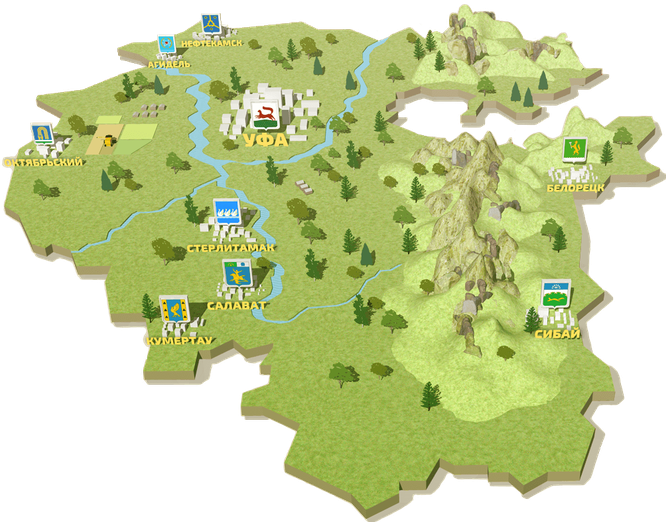
\includegraphics[width=85mm]{pics/alina/map.png}}
		\caption{Карта республики Башкортостан}
	\end{center}
\end{figure}

\end{frame}
%%%%%%%%%%%%%%%%%%%%%%%%%%%%%%%%%%%%%%%%%%%%%%%%%%%%%%%%%%%%%%%%%%%%

%%%%%%%%%%%%%%%%%%%%%%%%%%%%%%%%%%%%%%%%%%%%%%%%%%%%%%%%%%%%%%%%%%%%
\begin{frame}
\frametitle{Экономико-географического положение}

\begin{figure}[h!]
	\begin{center}
		{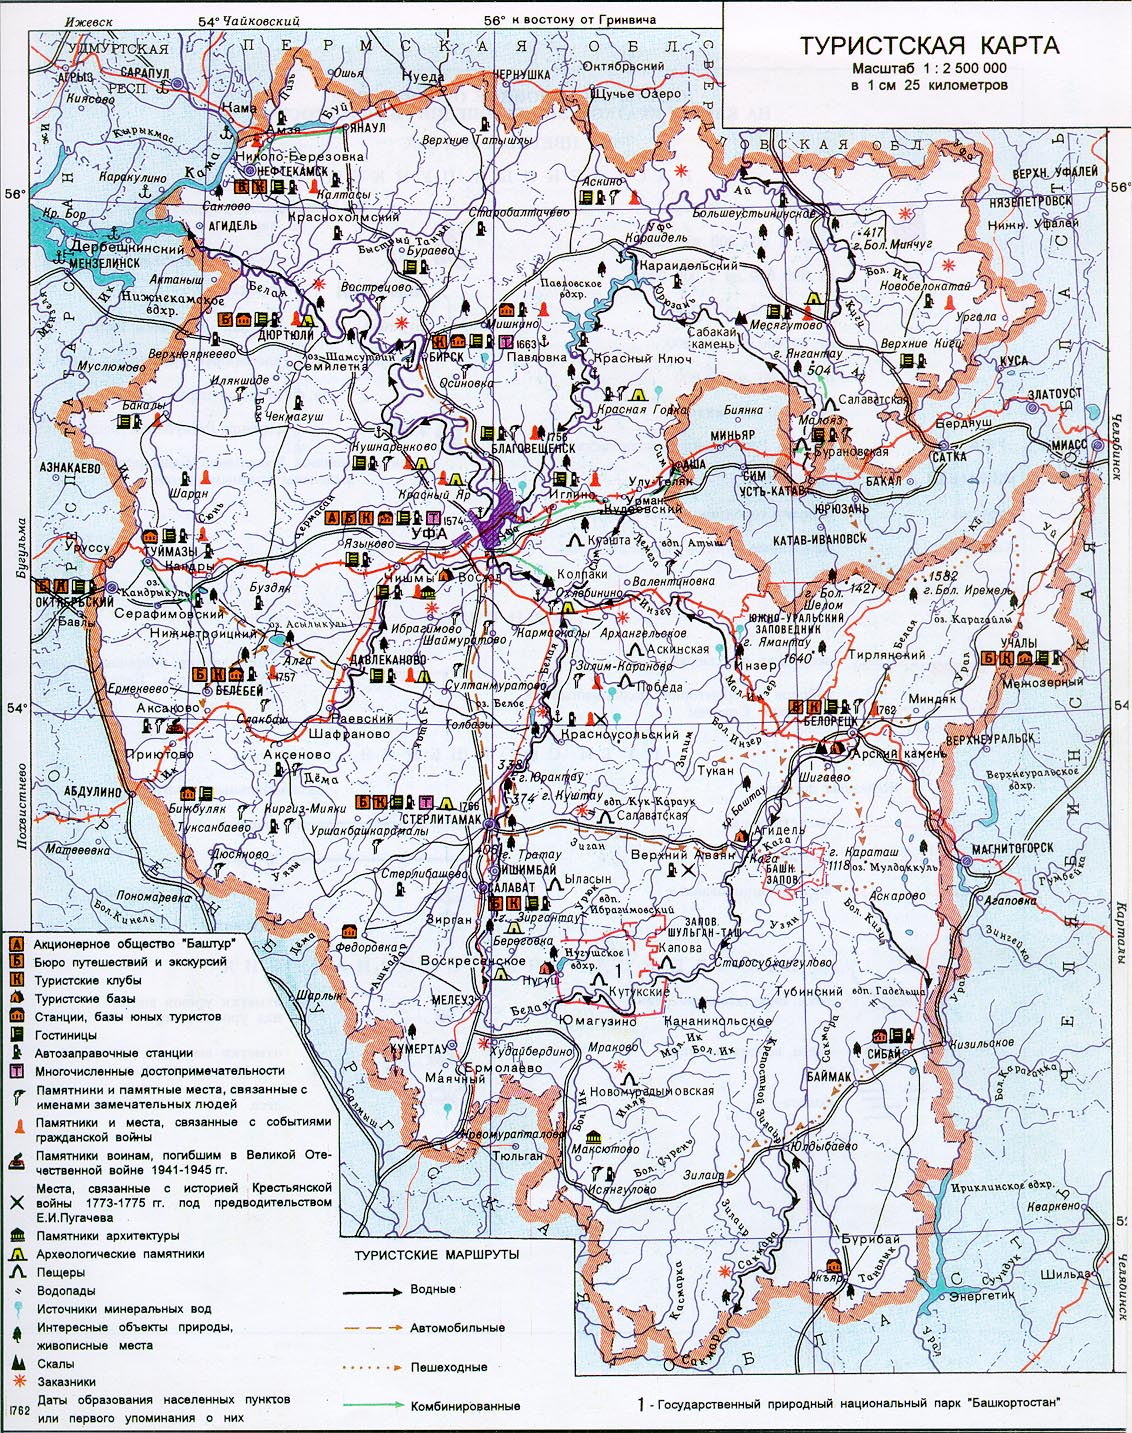
\includegraphics[width=60mm]{pics/alina/doroga.jpg}}
		\caption{Карта дорог республики Башкортостан}
	\end{center}
\end{figure}

\end{frame}
%%%%%%%%%%%%%%%%%%%%%%%%%%%%%%%%%%%%%%%%%%%%%%%%%%%%%%%%%%%%%%%%%%%%

%%%%%%%%%%%%%%%%%%%%%%%%%%%%%%%%%%%%%%%%%%%%%%%%%%%%%%%%%%%%%%%%%%%%
\begin{frame}
\frametitle{Экономико-географического положение}

\begin{figure}[h!]
	\begin{center}
		{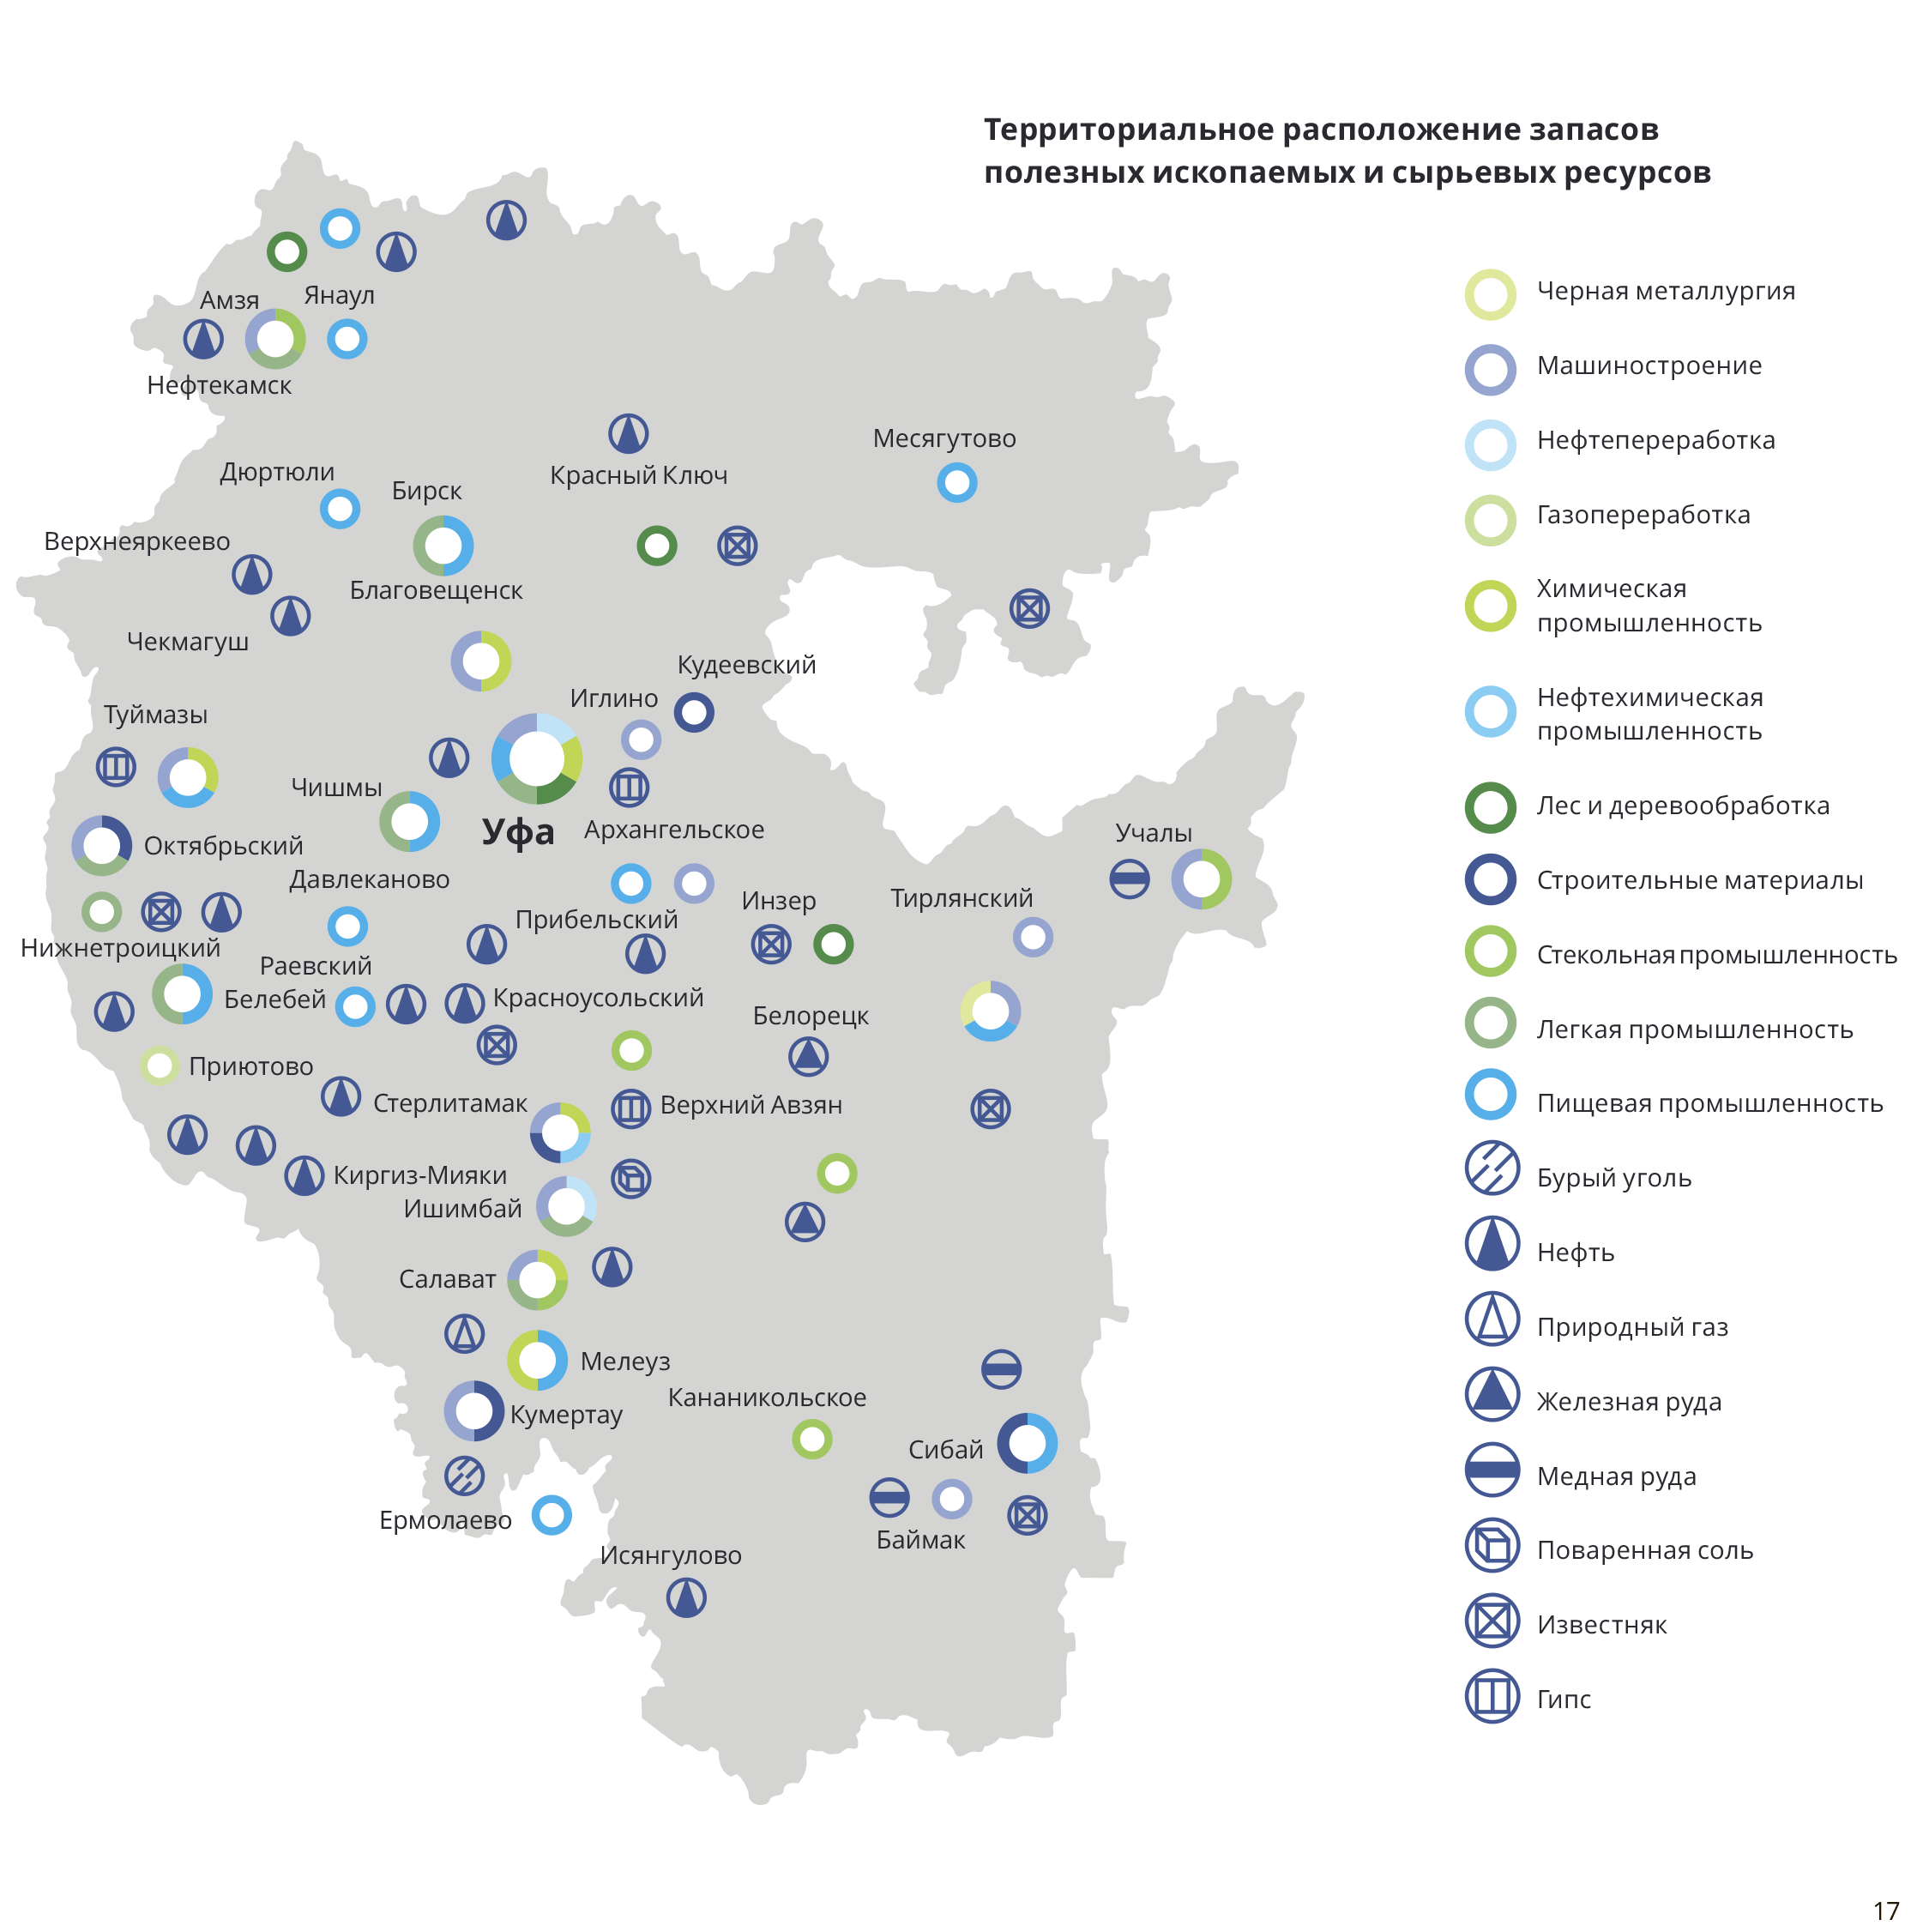
\includegraphics[width=85mm]{pics/alina/resource.png}}
	\end{center}
\end{figure}

\end{frame}
%%%%%%%%%%%%%%%%%%%%%%%%%%%%%%%%%%%%%%%%%%%%%%%%%%%%%%%%%%%%%%%%%%%%

%%%%%%%%%%%%%%%%%%%%%%%%%%%%%%%%%%%%%%%%%%%%%%%%%%%%%%%%%%%%%%%%%%%%
\begin{frame}
\frametitle{Административно-территориальная структура
	региона}

Современное административно-территориальное устройство Башкортостана регулируется Законом «Об административно-территориальном устройстве Республики Башкортостан» от 20 апреля 2005 года № 178-з. Во исполнение статьи 16 данного закона утверждён Реестр административно-территориальных единиц и населённых пунктов Республики Башкортостан.

\end{frame}
%%%%%%%%%%%%%%%%%%%%%%%%%%%%%%%%%%%%%%%%%%%%%%%%%%%%%%%%%%%%%%%%%%%%

%%%%%%%%%%%%%%%%%%%%%%%%%%%%%%%%%%%%%%%%%%%%%%%%%%%%%%%%%%%%%%%%%%%%
\begin{frame}
\frametitle{Административно-территориальная структура
	региона}

\begin{figure}[h!]
	\begin{center}
		{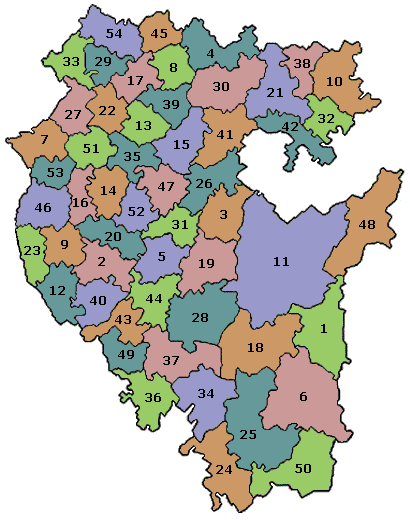
\includegraphics[width=50mm]{pics/alina/admin.png}}
		\caption{Районы Башкоростана}
	\end{center}
\end{figure}

\end{frame}
%%%%%%%%%%%%%%%%%%%%%%%%%%%%%%%%%%%%%%%%%%%%%%%%%%%%%%%%%%%%%%%%%%%%

%%%%%%%%%%%%%%%%%%%%%%%%%%%%%%%%%%%%%%%%%%%%%%%%%%%%%%%%%%%%%%%%%%%%
\begin{frame}
\frametitle{Административно-территориальная структура
	региона}

\begin{itemize}
	\item районы — 54
	\item внутригородские районы г. Уфы — 7
	\item рабочие посёлки (посёлки городского типа) — 2
	\item сельсоветы — 828
	\item сельские населенные пункты — 4538
\end{itemize}

\end{frame}
%%%%%%%%%%%%%%%%%%%%%%%%%%%%%%%%%%%%%%%%%%%%%%%%%%%%%%%%%%%%%%%%%%%%

%%%%%%%%%%%%%%%%%%%%%%%%%%%%%%%%%%%%%%%%%%%%%%%%%%%%%%%%%%%%%%%%%%%%
\begin{frame}
\frametitle{Административно-территориальная структура
	региона}

\begin{figure}[h!]
	\begin{center}
		{
\includegraphics[width=55mm]{pics/alina/spravka.png}}
		\caption{Официальный справочник «Административно - территориальное устройство Республики Башкортостан»}
	\end{center}
\end{figure}

\end{frame}
%%%%%%%%%%%%%%%%%%%%%%%%%%%%%%%%%%%%%%%%%%%%%%%%%%%%%%%%%%%%%%%%%%%%


\begin{frame}{Структура органов власти}

\insertpicc{emil/vlast.jpg}
    
\end{frame}

\begin{frame}{Дом республики}

\insertpicc{emil/adminka.jpg}
    
\end{frame}

\begin{frame}{Первый президент республики Башкортостан}

\begin{figure}[h!]
	\begin{center}
		{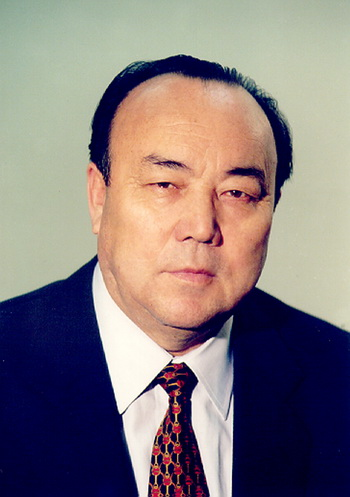
\includegraphics[width=0.5\linewidth]{emil/M_G_Rakhimov.jpg}}
		\caption{Районы Башкоростана}
	\end{center}
\end{figure}

\end{frame}


\begin{frame}{Первый президент республики Башкортостан}

\begin{figure}[h!]
	\begin{center}
		{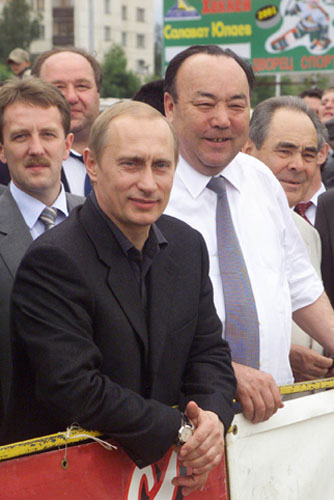
\includegraphics[width=0.4\linewidth]{emil/Murtaza_Rakhimov_and_Vladimir_Putin.jpg}}
		\caption{Муртаза Губайдулович Рахимов и Владимир Владимирович Путин}
	\end{center}
\end{figure}

\end{frame}

\begin{frame}{Заслуги}

\begin{itemize}
	\item Построено более 1000 школ
	\item В школах дети 15 национальностей имеют возможность изучать родной язык
	\item Республика входила в список регионов-доноров до 2006 года. И вновь вошла в список доноров в 2011 году, и входит в этот список до сих пор
	\item На июнь 2009 республика не входила в список кризисных
	\item За оказанную поддержку православной религии в республике Башкортостан, имя Муртазы Рахимова отлито на одном из колоколов собора Рождества Богородицы в Уфе
\end{itemize}

\end{frame}

\begin{frame}{Критика центральных властей}

\begin{itemize}
	\item Муртаза Рахимов о партии «Единая Россия»: «Партией пытаются рулить люди, которые и тремя курицами не командовали»
	\item Муртаза Рахимов: «С регионами легко стали делиться социальными обязательствами перед людьми, но не доходами»
\end{itemize}

\end{frame}

\begin{frame}{Что имеем на самом деле}

В России лишь чуть более десятка субъектов федерации обладает собственным крупным нефтяным потенциалом – только в 12 регионах добывается 10 и более миллионов тонн нефти в год.

\begin{itemize}
	\item среднедушевые доходы в последние 20 лет всегда были и есть ниже среднероссийских: по этому показателю республика занимает 22-е место в стране
	\item  по среднемесячному размеру назначенных пенсий республика на 60-м (!) месте среди субъектов Российской Федерации.
	\item по социальному расслоению Башкирия на седьмом месте в России, коэффициент дифференциации доходов 18,5, против 16,9 в среднем по России
\end{itemize}

\end{frame}

\begin{frame}{Что имеем}

\begin{figure}[h!]
	\begin{center}
		{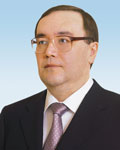
\includegraphics[width=0.25\linewidth]{emil/RahimovUM.jpg}}
		\caption{Рахимов Урал, В 2005—2012 годы входил в список 200 богатейших бизнесменов России по версии журнала Forbes}
	\end{center}
\end{figure}

После смены собственника «Башнефти» наблюдается взрывной рост платежей по налогу на прибыль: по данным компании за первый квартал 2010 года, они выросли в сравнении с I кварталом 2009 года в 12 (!) раз, что позволяет оценить масштаб занижения налога на прибыль в предыдущие годы. 
\end{frame}

\begin{frame}{Второй президент республики Башкортостан}

\begin{figure}[h!]
	\begin{center}
		{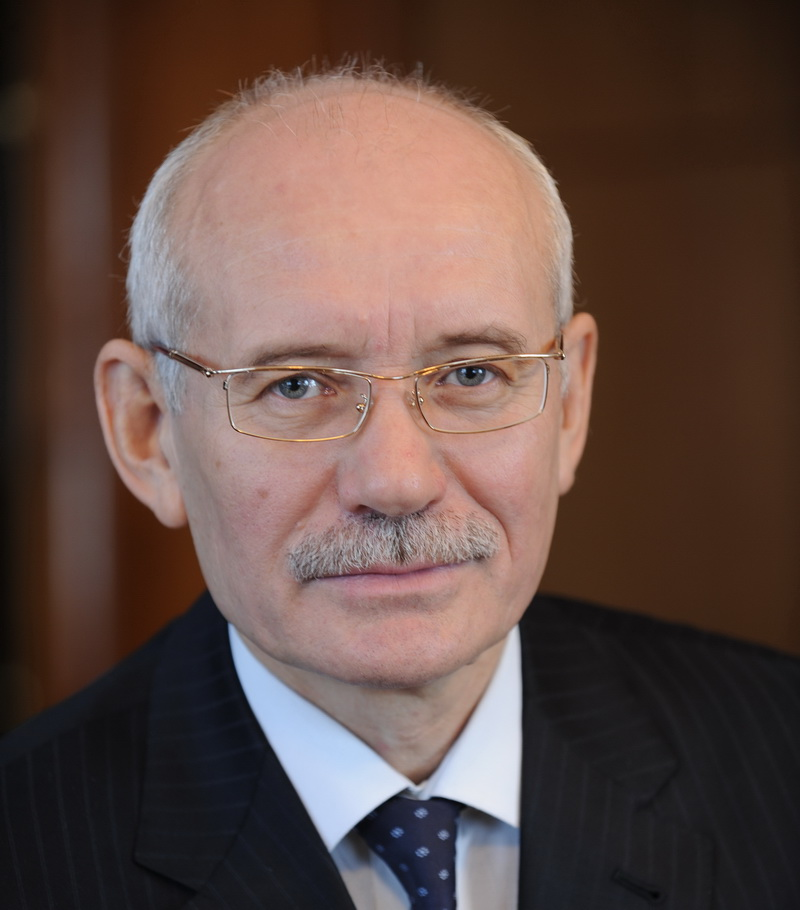
\includegraphics[width=0.5\linewidth]{emil/Rustem_Khamitov.jpg}}
		\caption{Хамитов Рустэм Закиевич}
	\end{center}
\end{figure}

\end{frame}

\begin{frame}{Положительные моменты правления}

\begin{itemize}
	\item  ВРП региона вырос с 759,2 млрд рублей в 2010 году до 1 трлн 343,9 млрд в 2014
	\item уменьшилась доля добычи полезных ископаемых в структуре валового продукта региона, если в 2009 году она составляла 8,1 \%67, то в 2012 году уже 2,9 \%68
	\item спустя 10 месяцев после вступления Рустэма Хамитова в должность Президента Башкортостана, международное рейтинговое агентство Standard \& Poor’s (S\&P) повысило долгосрочный кредитный рейтинг республики со «стабильного» (BB-) на «позитивный» (BB+)
	\item в 2012 году Башкортостан получил высшую оценку Национального рейтинга прозрачности закупок — «Гарантированная прозрачность», переместившись с 34-го места по этому показателю на второе
\end{itemize}
\end{frame}

\begin{frame}{Отрицательные моменты правления}

\begin{itemize}
	\item  в 2010 году долг составлял 6,9 млрд рублей (1 \% от ВРП), то к концу 2013 года он дошёл до 19,8 млрд рублей
	\item увеличение дефицита бюджета региона: в 2010 году — 3,4 млрд рублей; в 2014 — 15 млрд рублей
	\item  в период нахождения Хамитова на посту главы региона наблюдается отрицательный прирост населения, что может являться показателем неблагоприятной экономической ситуации
	\item регион из энергодостаточного превратился в энергодефицитный. Если в 2011 году потребление электроэнергии на 2,4 \% опережало производство, то в 2015 году наметился дефицит в 16,5 \%
	\item обострениt проблем с коррупцией, особенно в сфере ЖКХ
\end{itemize}

\end{frame}



%%%%%%%%%%%%%%%%%%%%%%%%%%%%%%%%%%%%%%%%%%%%%%%%%%%%%%%%%%%%%%%%%%%%
\begin{frame}
	\begin{center}
		\Huge{\Blue{Спасибо за внимание!}}
	\end{center}
\end{frame}
%%%%%%%%%%%%%%%%%%%%%%%%%%%%%%%%%%%%%%%%%%%%%%%%%%%%%%%%%%%%%%%%%%%%

\end{document}
